\documentclass[../Main.tex]{subfiles}
\begin{document}


This section describes functionality and design principles of implemented mobile application for style transfer. We present the whole application, screen by screen, and some of the difficulties we were facing during development.

\subsection{Requirements}
During planning process we decided that our application ought to meet all of the 
undermentioned requirements.
User should be able to:
\begin{itemize}
    \item manage filters in the gallery, where it is easy to pick filter image
    \item take photo directly inside the application and then use it as a filter
    \item set style transfer settings - like color preservation or scaling
    \item transfer style from filter to a real-time video
\end{itemize}

\subsection{Design}
Our assumption was to fill the application with marvelous image content.
We used the greatest artworks from Wikiart \cite{wikiart} so a user should \textit{feel communication} with the real art.
To achieve this goal we let images take the whole screen and put them in the foreground.
Most of the UI elements are transparent at some level so they do not cover the images.
Buttons and icons are very subtle as well as kept in Google Material Design style.
Animations are also gentle and they are introduced in order to improve user's experience rather than make spectacular visual effects.


\subsection{Difficulties}
To perform style transfer with application and meet all of the requirements
we had to overcome two main difficulties:
\begin{itemize}
    \item sending video to server and then receiving it back with applied style transfer (real-time streaming)
    \item implementing efficient image gallery which can load photos from smartphone's storage
\end{itemize}

Our main concept of this project was real-time streaming, so solving first problem was crucial.
A great, relatively new tool for streaming video is WebRTC which, in general, enables real-time communication in browser. 
Someone may wonder how this can allow us to stream video in a mobile application.
Actually, we use special Flutter \href{https://pub.dev/packages/flutter_inappwebview}{InAppWebView} plugin which can display websites inside application.
With this plugin we are able to move almost all logic associated with communication into server.
The application is just opening website under hardcoded specific address.

As mentioned, the second task is to create an effective custom image gallery. 
Most smartphones take high resolution pictures which size is around 3-4 MB.
It takes long time for Flutter to load big pictures like these, especially when
we have to load twelve or even more photos. We need to load plenty of of pictures, but they could be in fact very small since they ought to be presented as the thumbnails.
In addition, there is a problem with 
memory overflow. Namely when we are loading all pictures at once application was
crashing after few second. 
So as, to face memory overflow and high loading times, we apply two key improvements:
lazy loading and image resize in line with compression.
The gallery loads only twelve pictures at the same time so memory will not be filled so quickly.
The improved gallery is also resizing file to $400\times400$ resolution and then compression is applied.
Thus, it lets to save memory and time.


\subsection{Application walk-through}
This part presents final client application and all its capabilities.
Every screenshot comes from Huawei P10 Lite with Android 8.1 operating system. In the pictures we can see application design which was described in previous chapters.

\subsubsection{Start screen}
The star screen appears just after application is launched. It has only aesthetic purpose and is an introduction to the main part of the application. We can see here Vincent van Gogh picture \textit{Seascape near Les Saintes-Maries-de-la-Mer} and it is just one of the 27 pre-built image-filters. The screen also contains the application name \textit{ARTEXTURE}. If we would like to go to next screen we have to swipe up or tap arrow button at the bottom.


\begin{figure}[H]
    \centering
    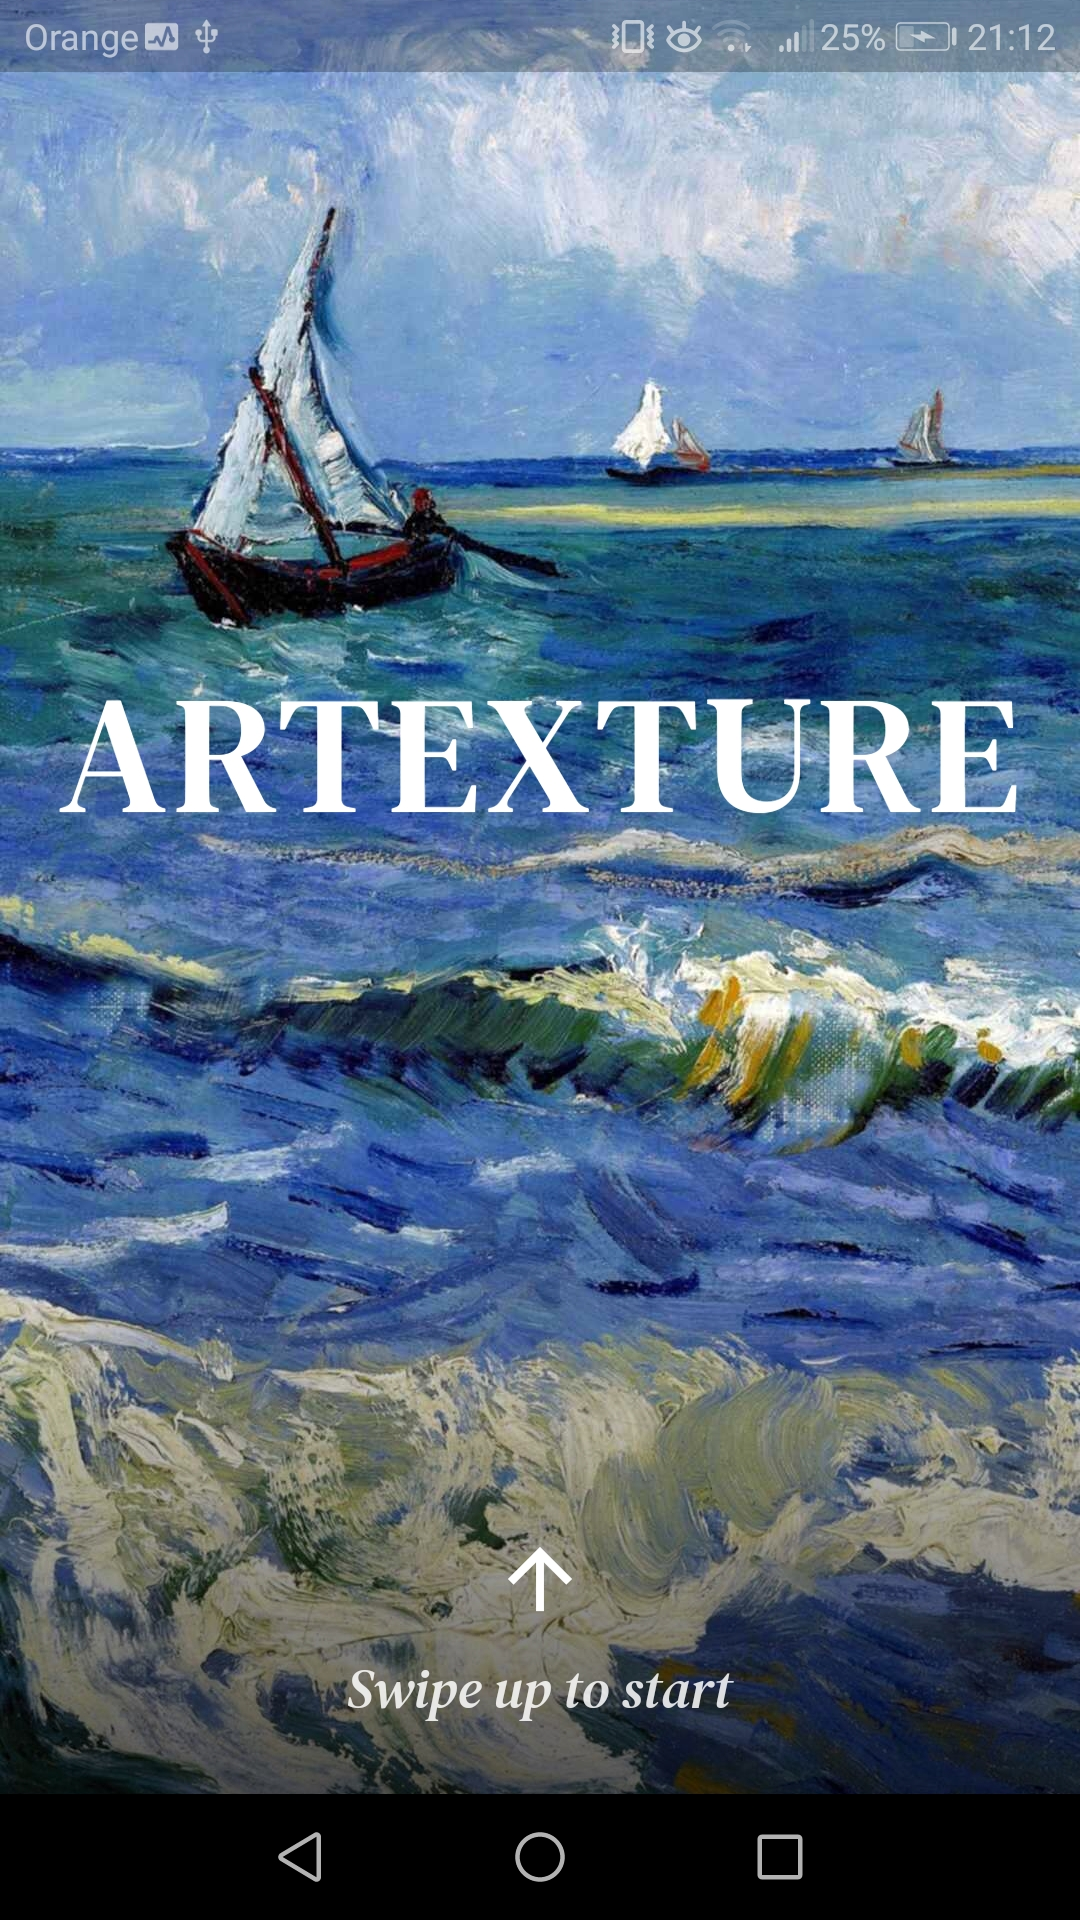
\includegraphics[width=0.325\textwidth]{start_screen.jpg}
    \caption{Start screen}
    \label{fig:start-screen}
\end{figure}


\subsubsection{Gallery}
The gallery is the main screen of the application. It allows us to pick an image 
that we want to use as a filter. The bottom half of the screen is taken by a list of images and it is presented in Figure \ref{fig:gallery_unfolded}.
There are 27 built-in paintings images built in the application. We can also use images from storage.
To switch between these two you have to click the pallet icon on the image icon on top of the list.
If we select one of the images from the list it appears immediately in the background.
In order to have a good look at the whole selected image, there is a possibility 
to hide the list by clicking on a down arrow icon (Figure \ref{fig:gallery_folded}).
In the right upper corner there is settings icon and after tapping we can see a 
alert box (Figure \ref{fig:gallery_options}) with two filter settings:
\textit{intensity} and \textit{color preservation}.
Next to the settings icon, there is a plus icon which leads us \textit{Pick a filter} 
to the screen which is described on the next pages.


\begin{figure}[H]
    \minipage{0.32\textwidth}
        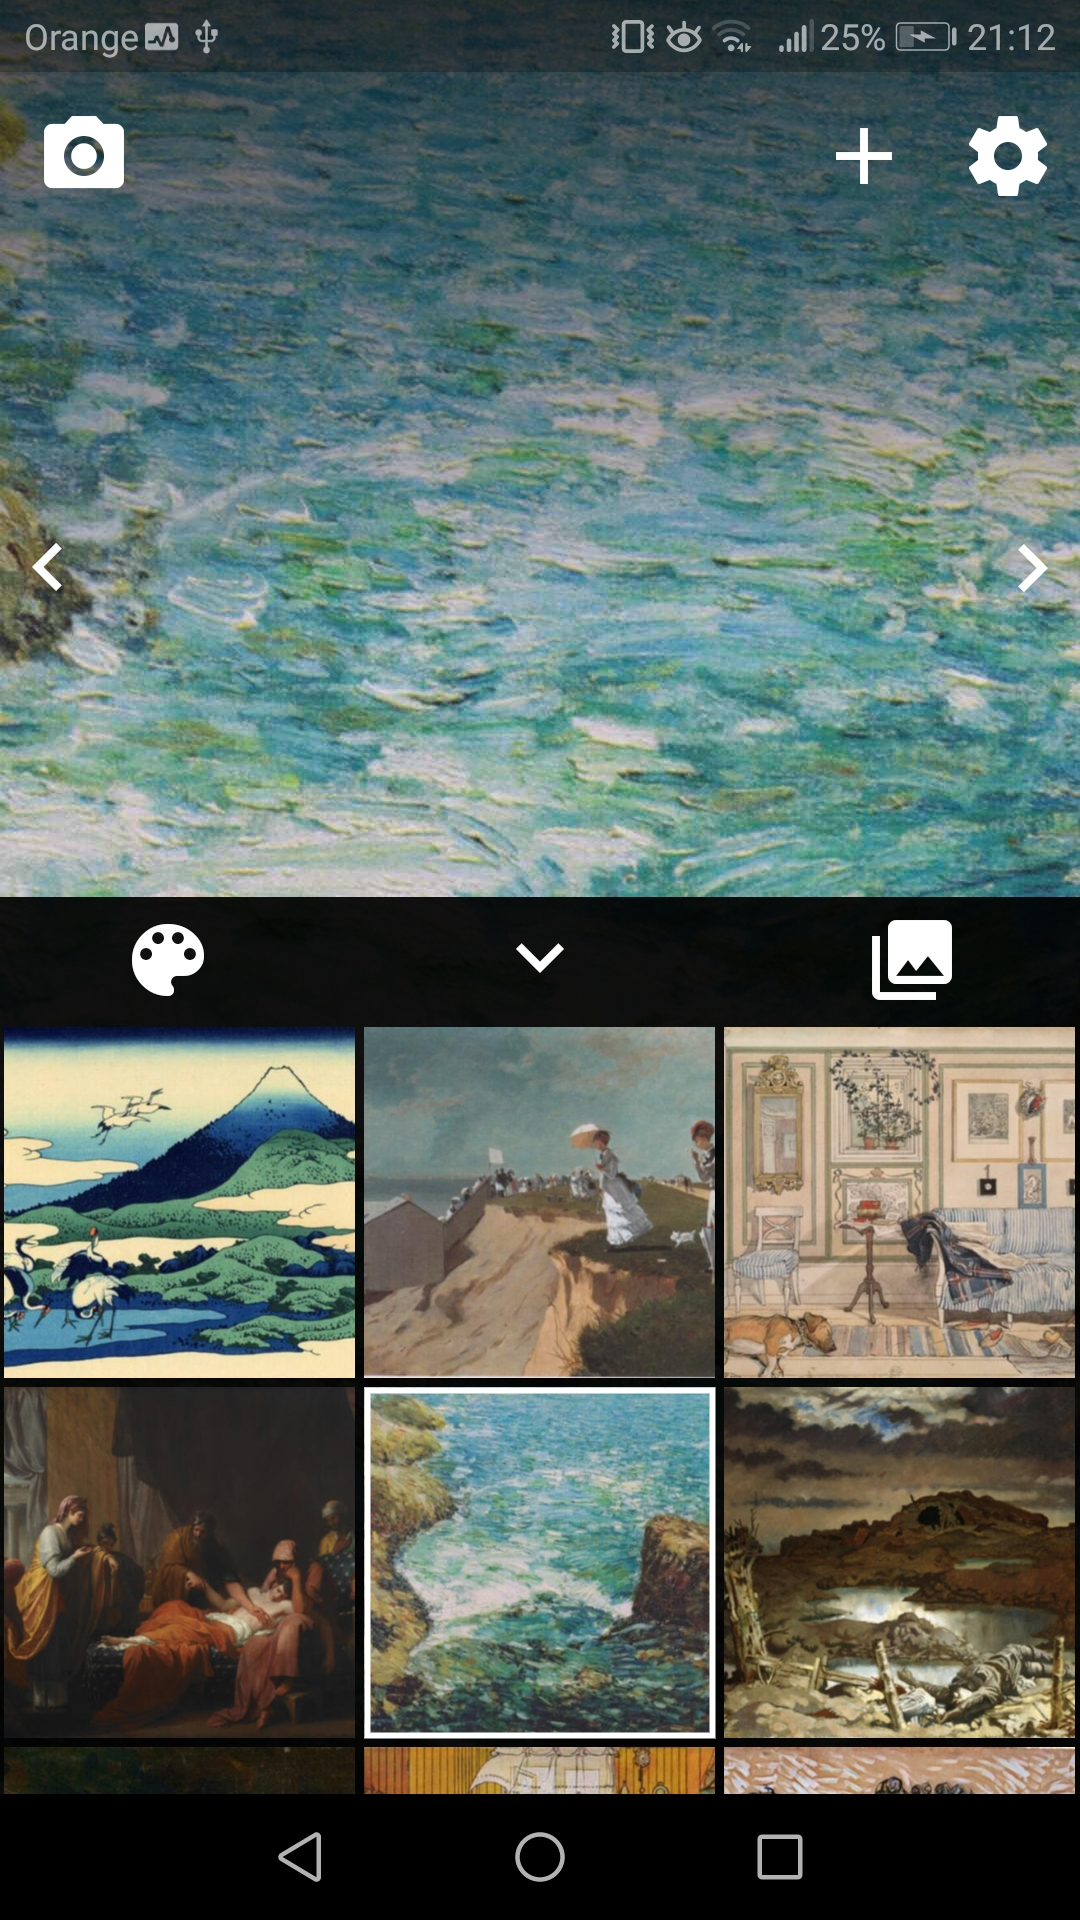
\includegraphics[width=\linewidth]{gallery_1.jpg}
        \caption{Unfolded gallery}\label{fig:gallery_unfolded}
    \endminipage\hfill
    \minipage{0.32\textwidth}
        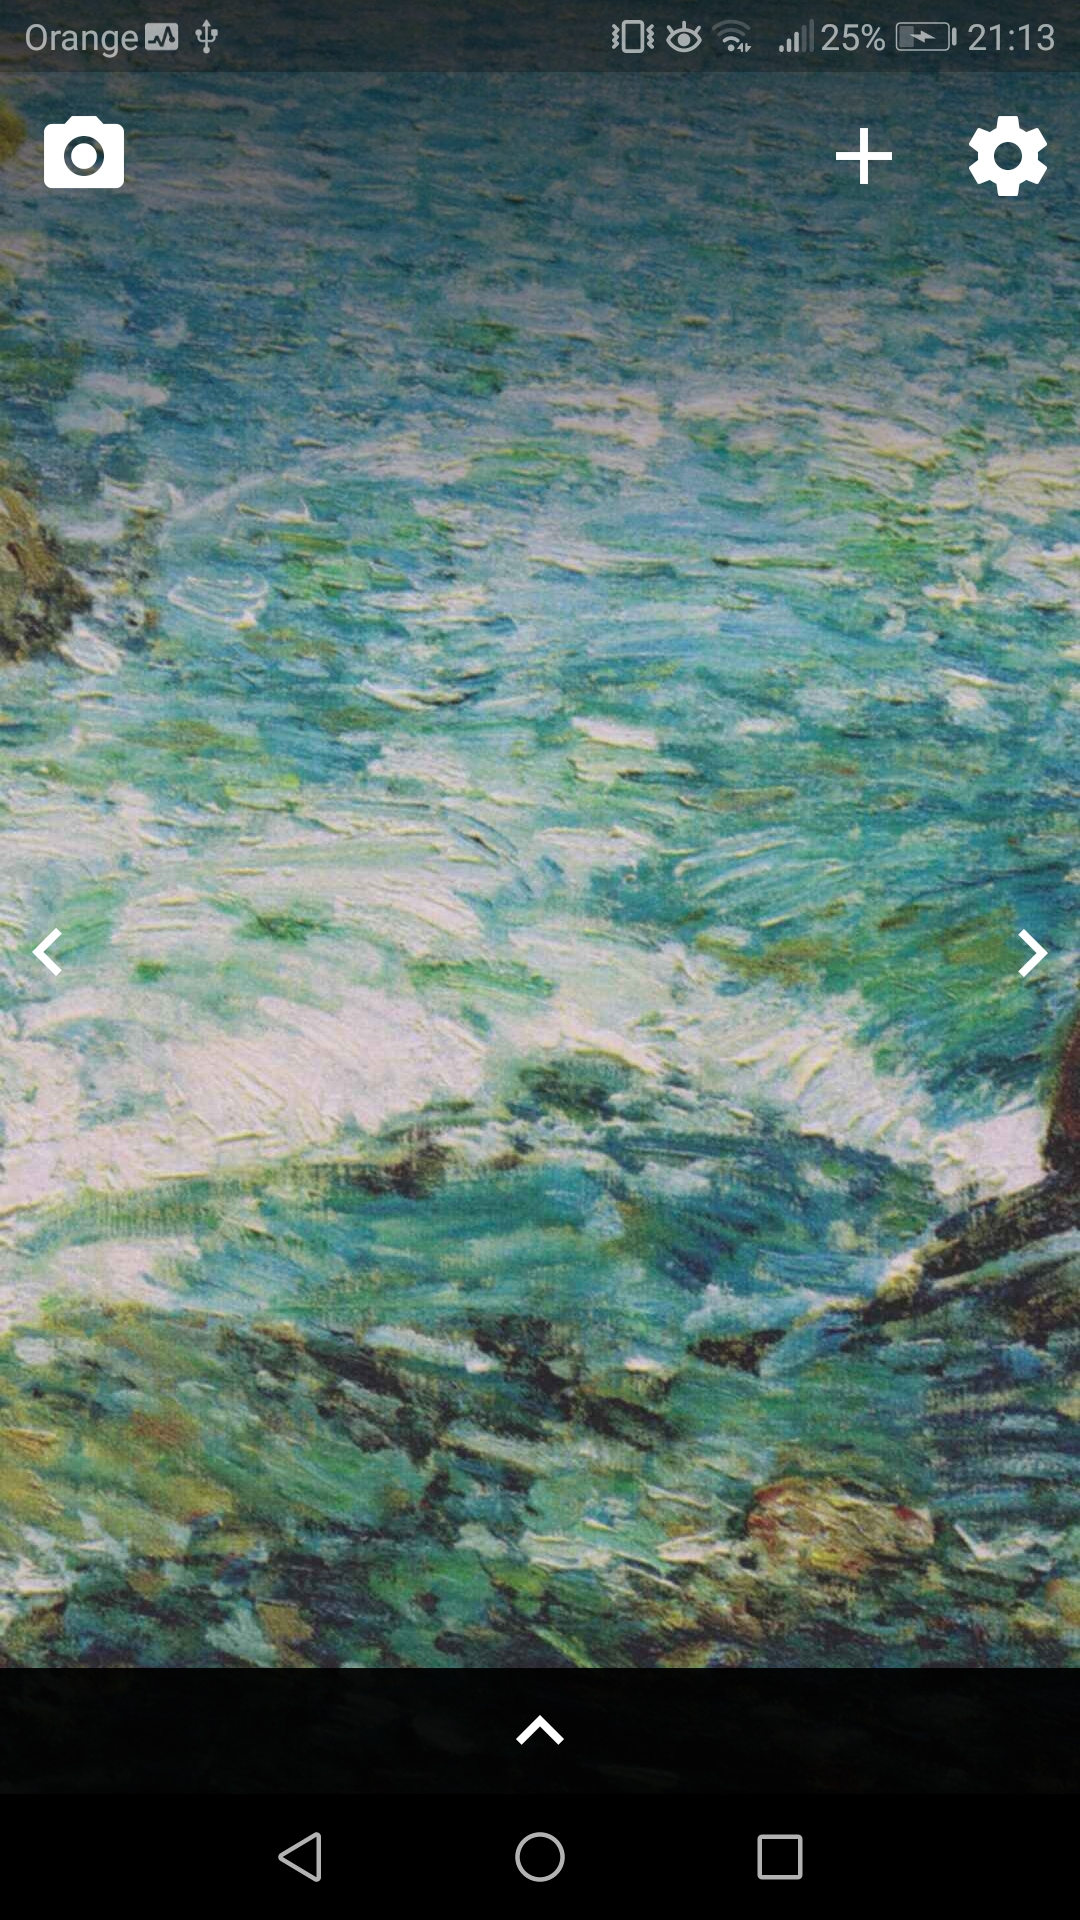
\includegraphics[width=\linewidth]{gallery_2.jpg}
        \caption{Folded gallery}\label{fig:gallery_folded}
    \endminipage\hfill
    \minipage{0.32\textwidth}
        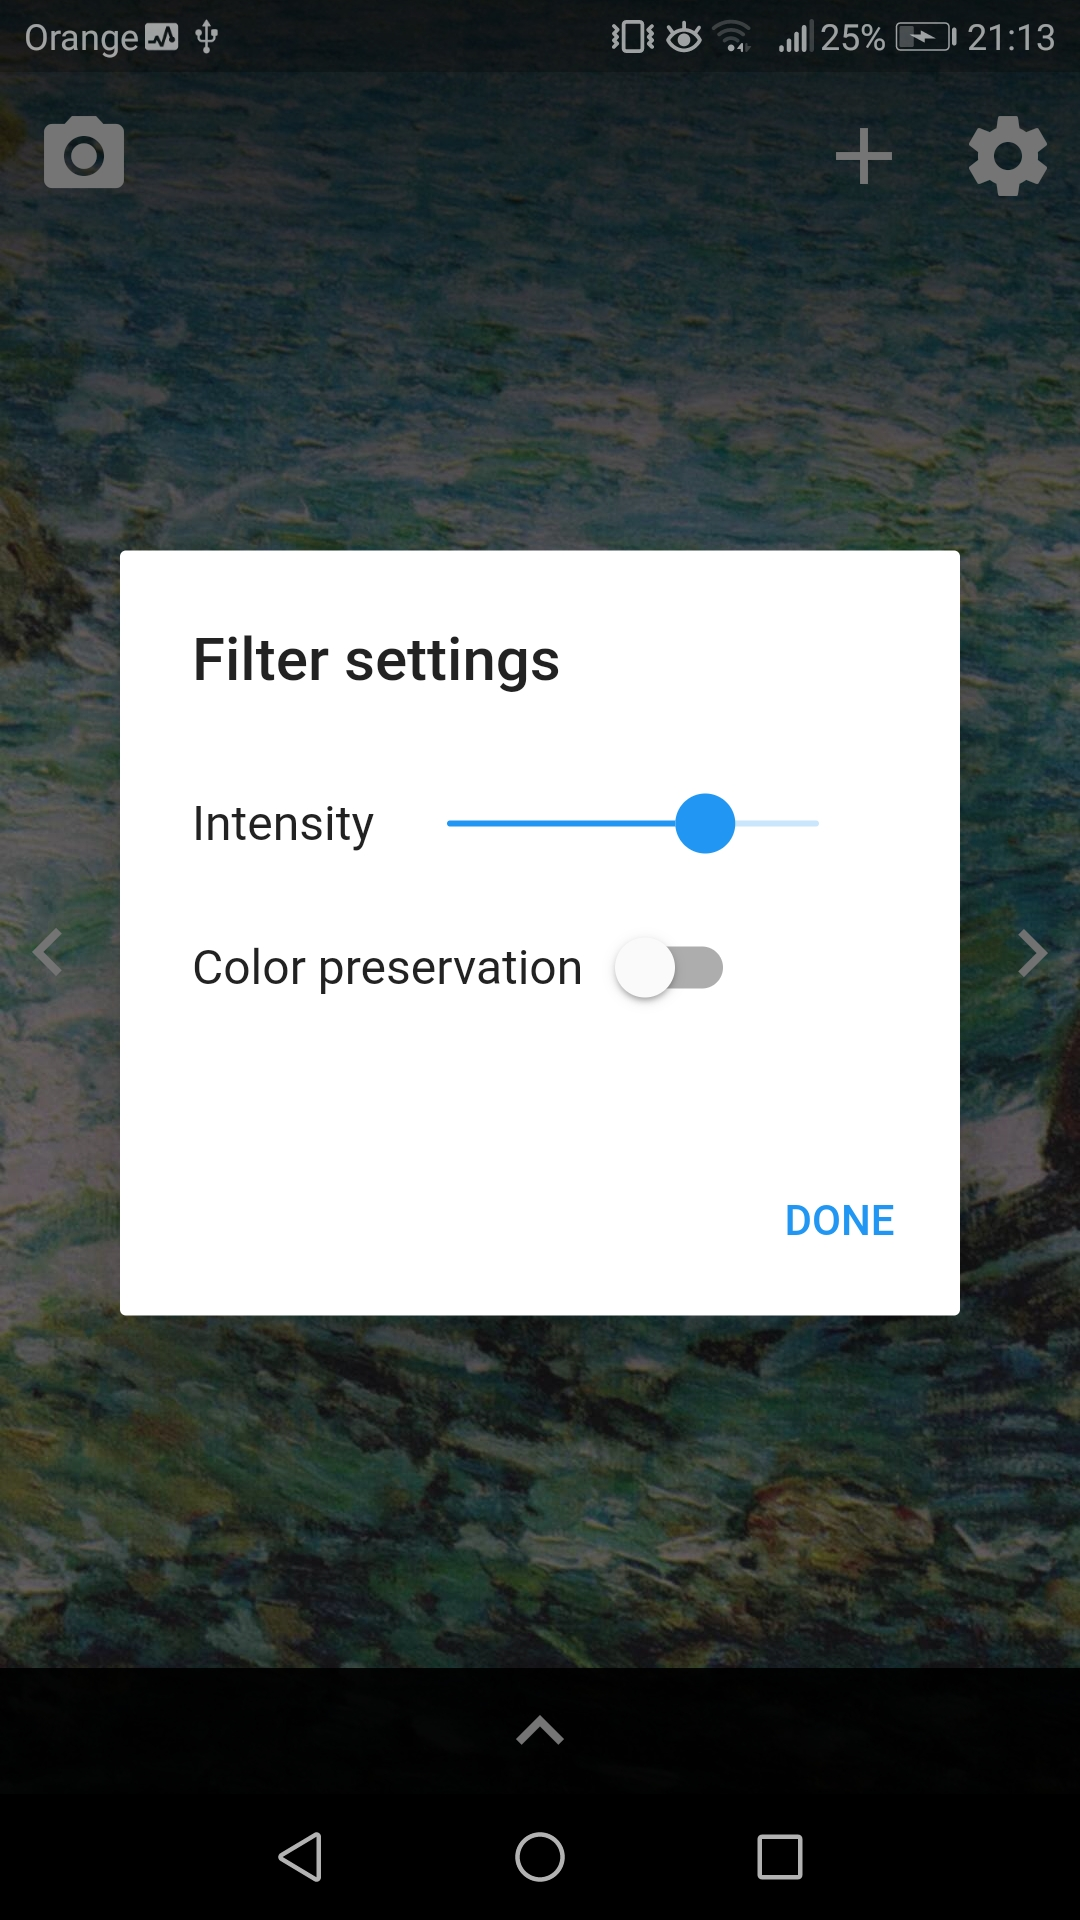
\includegraphics[width=\linewidth]{options.jpg}
        \caption{Settings}\label{fig:gallery_options}
    \endminipage\hfill
\end{figure}


\subsubsection{Style transfer screen}
When we finally pick our filter and settings we can start style transfer.
Whole screen screen is filled with transformed video.
If we do not like the current filter or we want to stop style transfer all we need to 
do is push \textit{X} button at the bottom of the screen.
Afterwards, we go back to the gallery. 

\begin{figure}[H]
    \minipage{0.32\textwidth}
        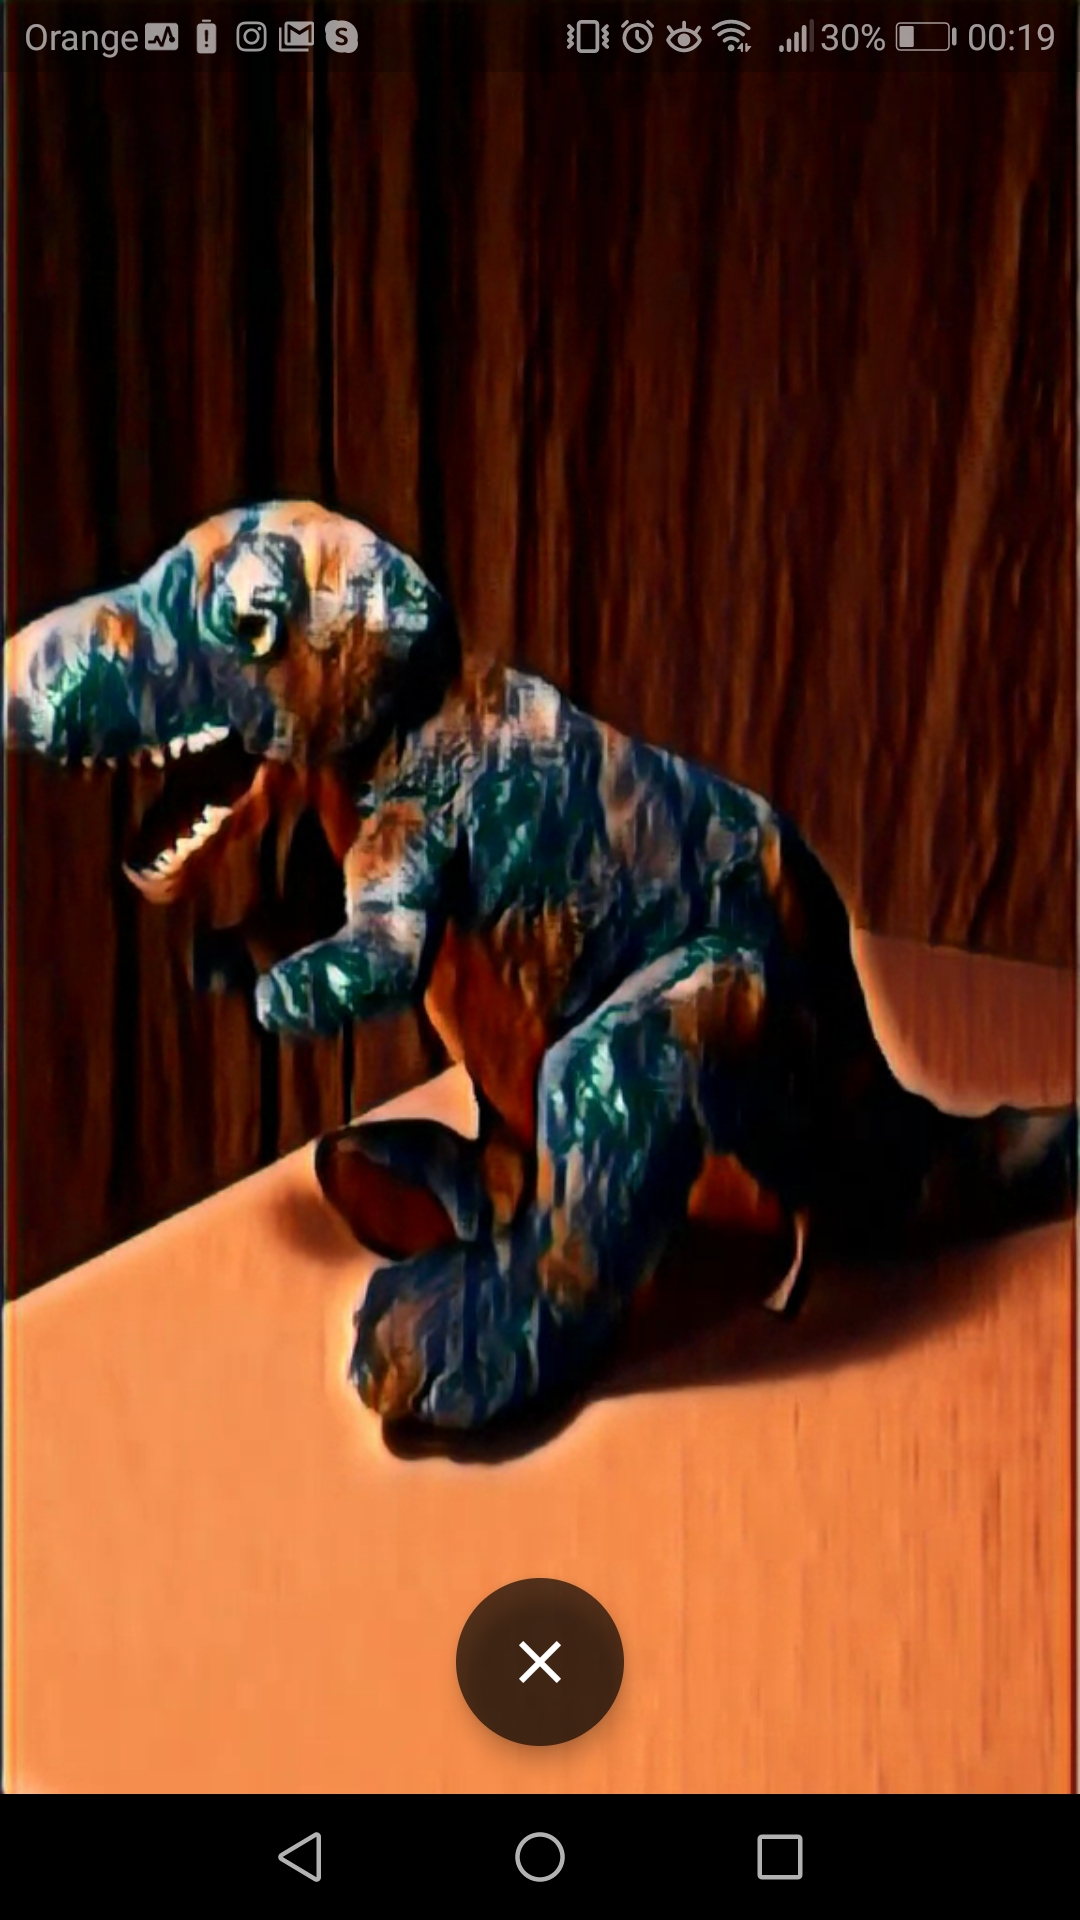
\includegraphics[width=\linewidth]{Images/app_photos/dino/twin.jpg}
    \endminipage\hfill
    \minipage{0.32\textwidth}
        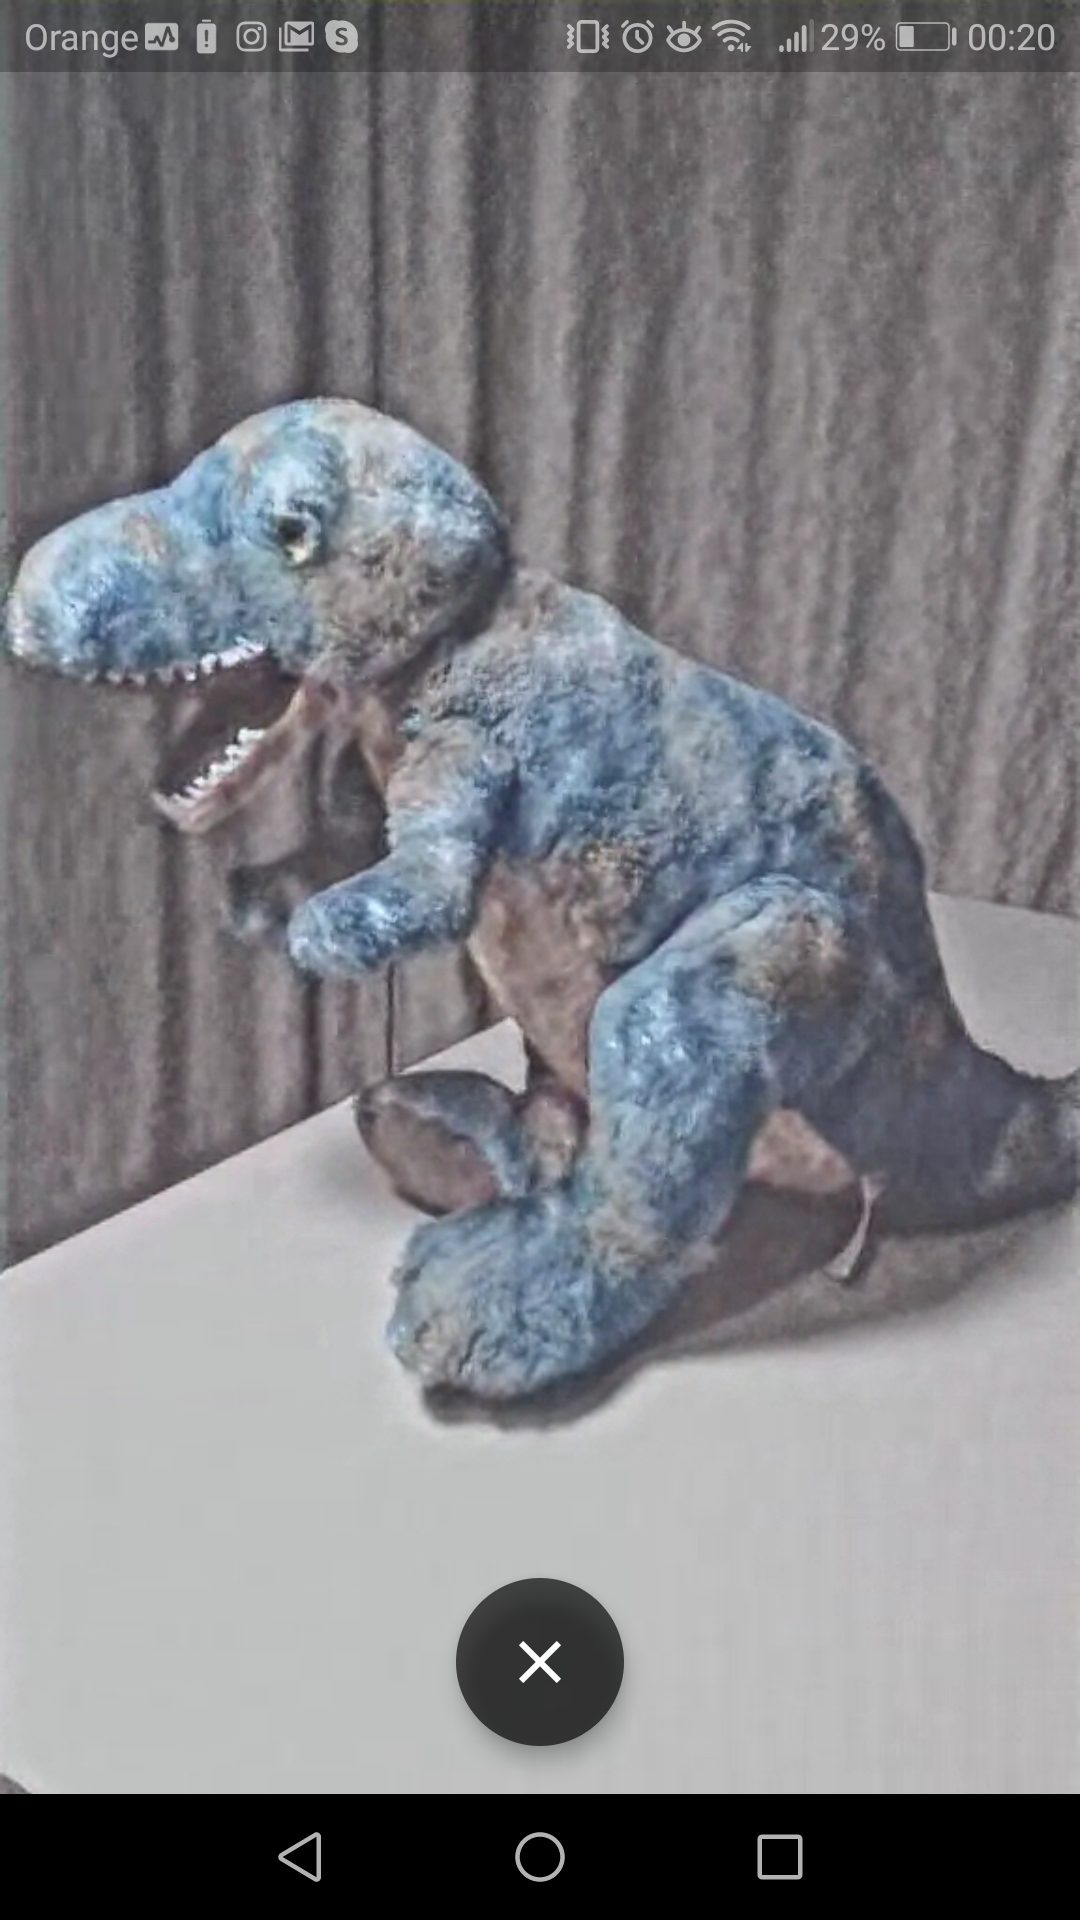
\includegraphics[width=\linewidth]{Images/app_photos/dino/draw.jpg}
    \endminipage\hfill
    \minipage{0.32\textwidth}
        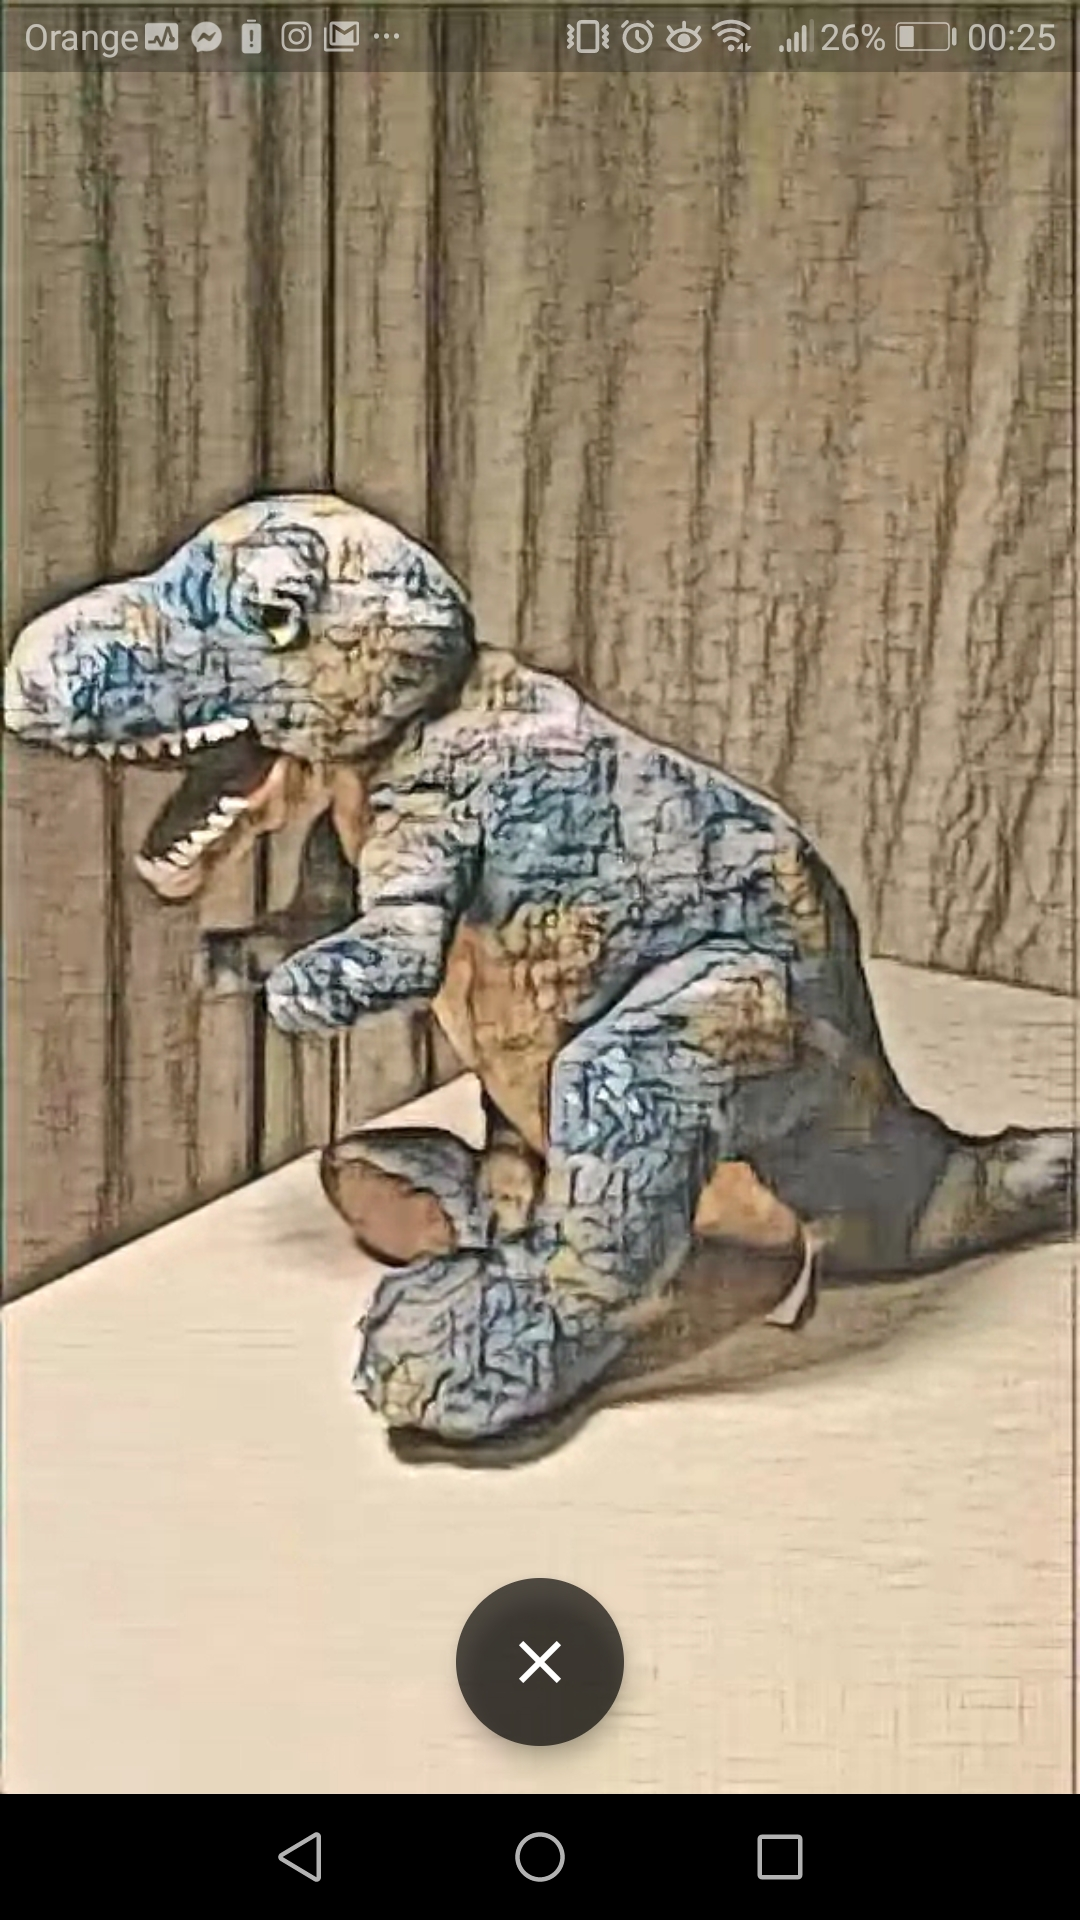
\includegraphics[width=\linewidth]{Images/app_photos/dino/salon.jpg}
    \endminipage\hfill
    \caption{Style transfer with different filters}\label{fig:gallery_options}
\end{figure}


\subsubsection{\textit{Pick a filter} screen}
While working on this project, we anticipated that there might be a situation that the users will notice a ravishing 
scenery or a breathtaking view. In these circumstances, they can use it as a filter.
There is an opportunity to pick a photo quickly and then start style transfer immediately.
In Figure \ref{fig:preview} we can see the camera preview from the back camera.
Users can also switch to front camera by clicking \textit{switch camera}
the icon in the top right corner.
After we take a picture we are redirected to the screen presented on Figure 
\ref{fig:taken_photo} and then we can decide whether to use the picked photo as a filter or not.
If we are satisfied with the filter image we have to press \textit{Style it} button.
After that, the style transfer begins.



\begin{figure}[H]
    \centerline{
    \minipage{0.32\textwidth}
        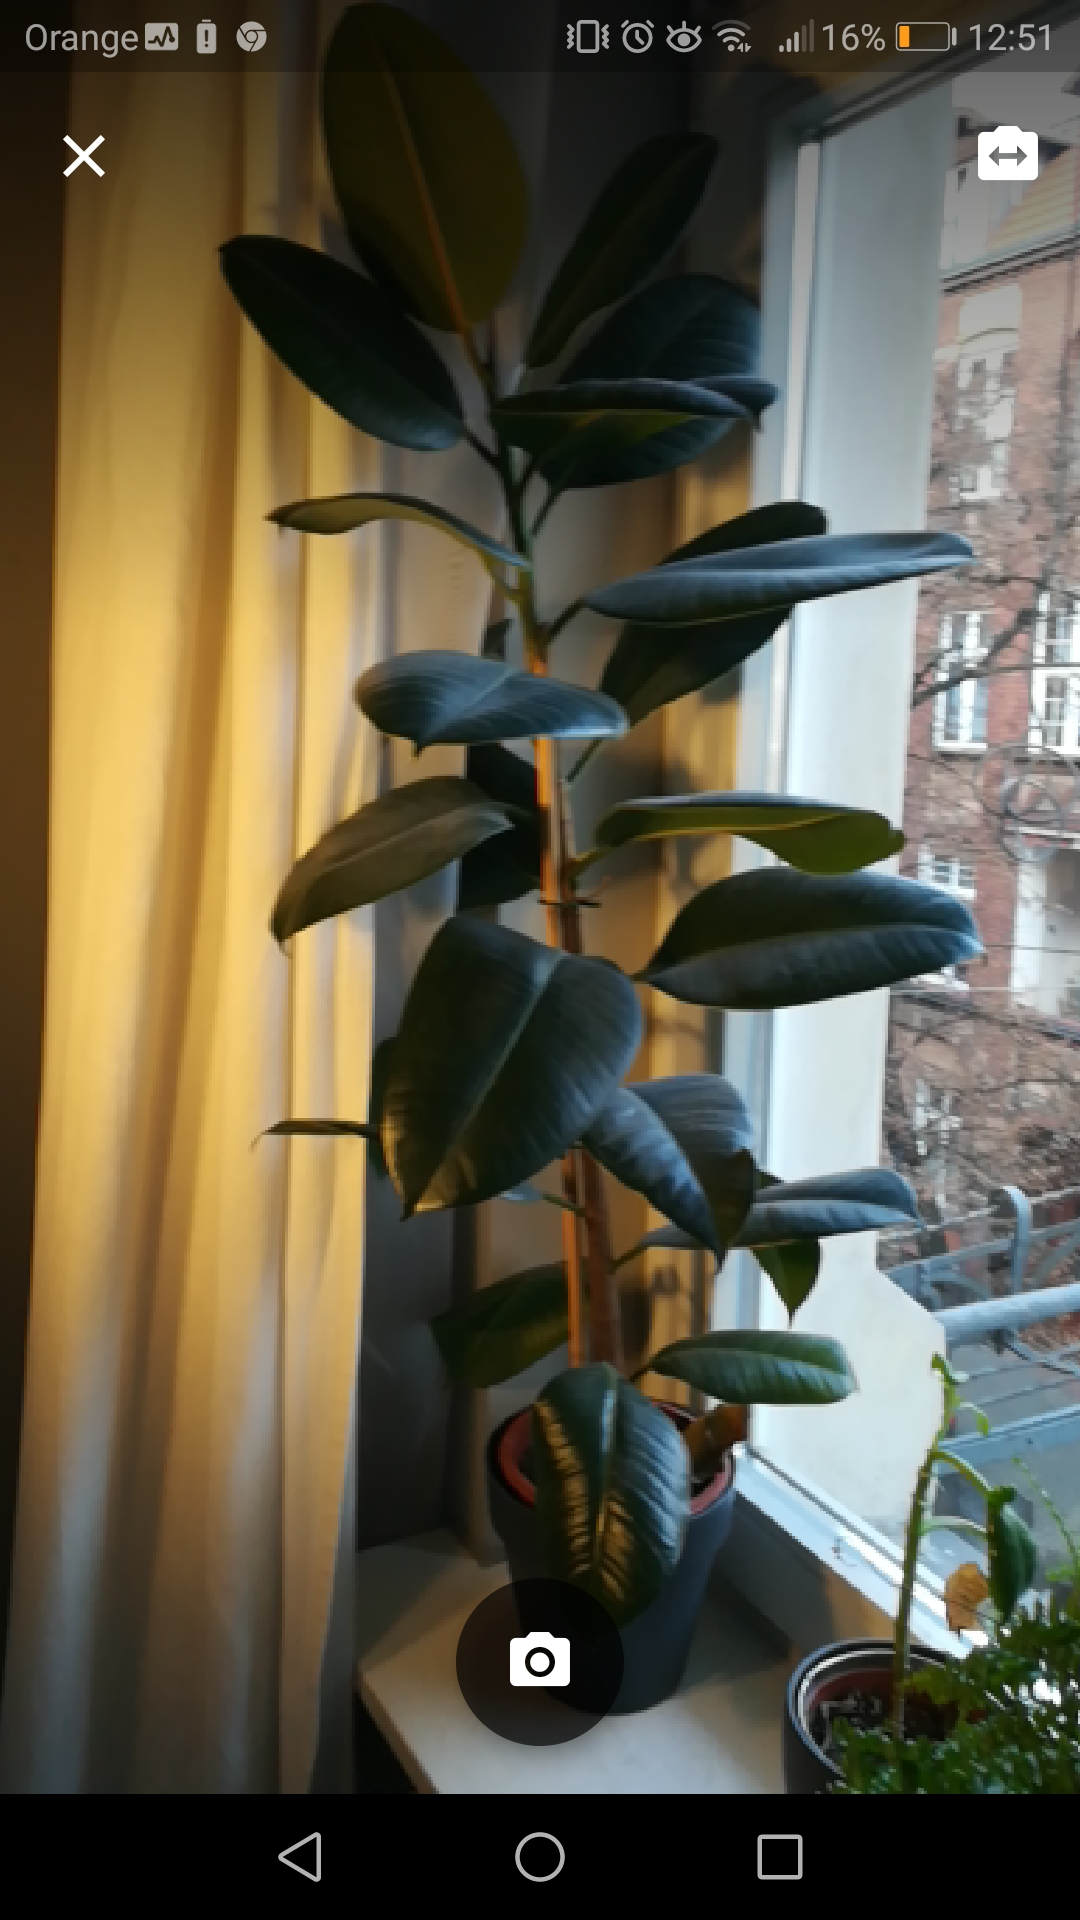
\includegraphics[width=\linewidth]{pick2.jpg}
        \caption{Camera preview}\label{fig:preview}
    \endminipage\hspace{0.01\textwidth}
    \minipage{0.32\textwidth}
        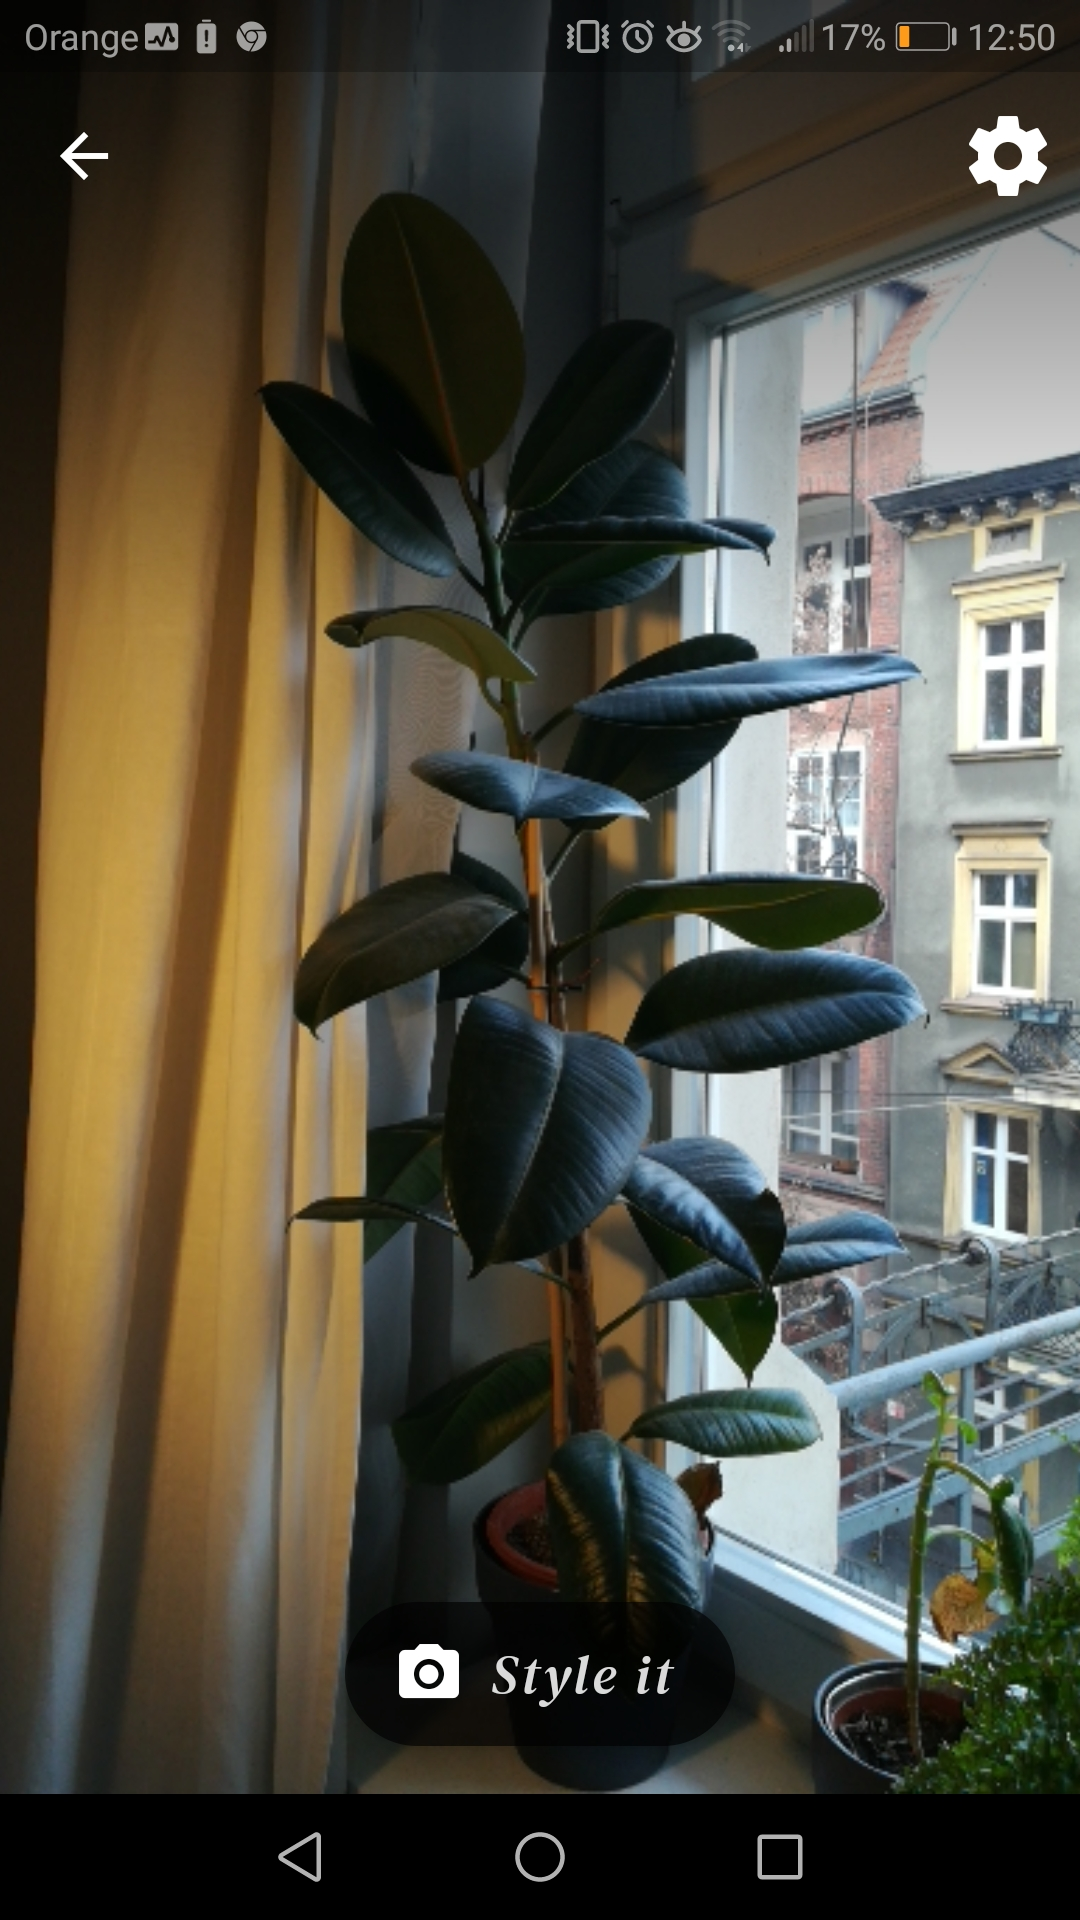
\includegraphics[width=\linewidth]{pick1.jpg}
        \caption{Taken photo}\label{fig:taken_photo}
    \endminipage}
\end{figure}



























\end{document}
